\section{Overview}

GEMC \cite{gemc} is a c++ framework that uses geant4 \cite{geant4} to simulate the passage of particles through matter. It provides:
\begin{itemize}
	\item application independent geometry description
	\item easy interface to build / run experiments
	\item cad/gdml imports
\end{itemize}

The simulation parameters are stored in external databases and are used to define the geant4 objects at run time. This includes:
\begin{itemize}
	\item geometry
	\item materials
	\item mirrors
	\item physics list
	\item database constants
	\item digitization
	\item electromagnetic fields
\end{itemize}

Particles are transported through matters and produce radiation, hits, secondaries.
gemc then collects the geant4 results and produce the output specified by the user.
The design of the framework is summarized in \F{gemcDesign}

\begin{figure}
	\centering
	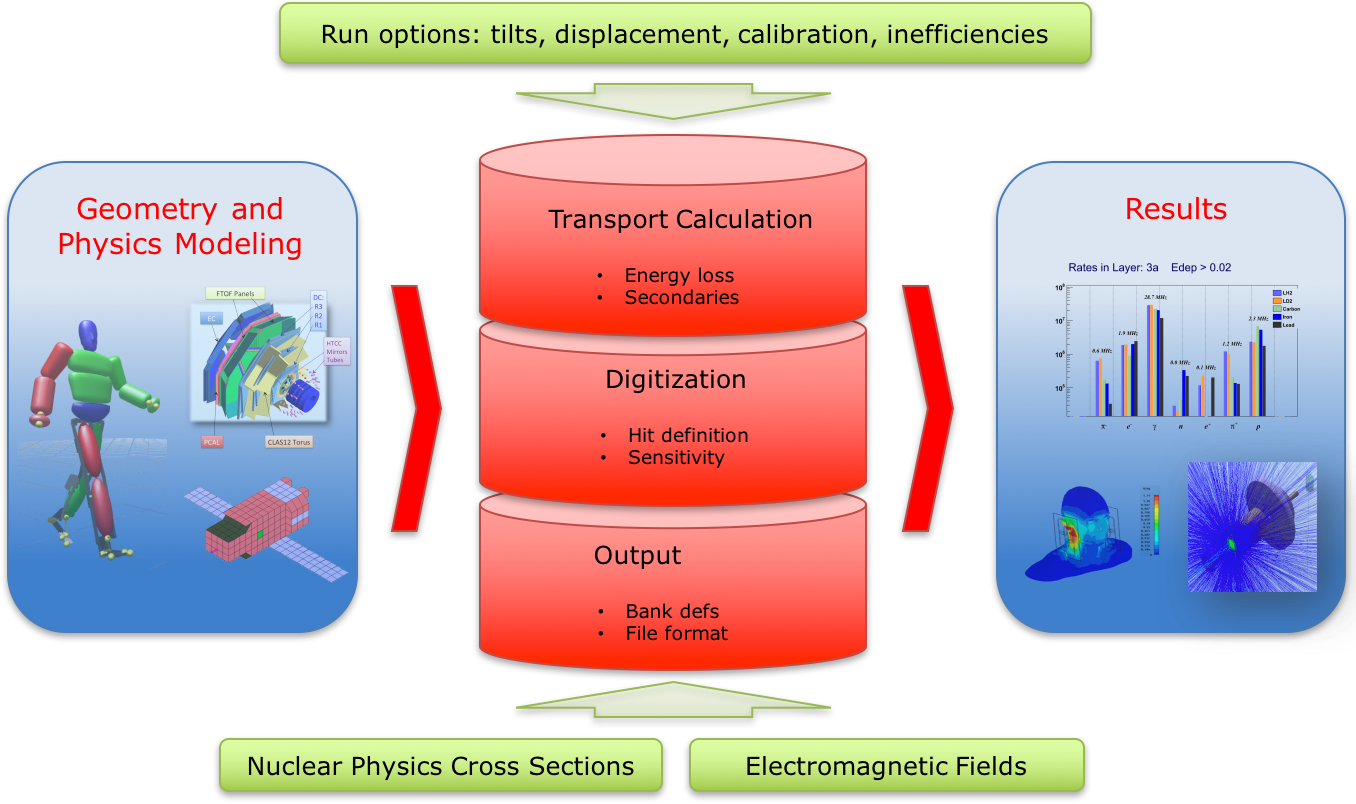
\includegraphics[width=0.98\columnwidth,keepaspectratio]{img/gemcDesign.png}
	\caption{The architecture of GEMC. The geant4 objects are defined in external database. geant4 is used to simulate the
             passage of particles through materials, and hits are digitized with plugins defined by users
             and collected in user-defined outputs. }
	\label{fig:gemcDesign}
\end{figure}


\subsection{Geometry and Materials Import}

The geometry and material are stored extrnal databases that can be mysql tables or text files that mimic the mysql tables.
The databases can be defined using the following factories:

\begin{itemize}
	\item gemc native api (perl or python)
	\item geometry service
	\item cad (stl, ply, obj formats)
	\item gdml, c++ plugins (not used in CLAS12)
\end{itemize}

The gemc native api repository is \url{https://github.com/gemc/api}. The geometry service code repository is
\url{https://github.com/JeffersonLab/clas12-offline-software/blob/development/common-tools/clas-jcsg/src/main/java/org/jlab/detector/geant4/v2/}


\subsubsection{Geometry database using native api or geometry service}

An example of the code to define and store a geant4 volume in external databases is shown below. The
numbers are typically hardcoded, come from a calibration databases or are defined in the geometry service. The material
has a similar interface.

\begin{lstlisting}[language=Perl]
my %detector = init_det();

$detector{"name"}        = "shield";
$detector{"mother"}      = "root";
$detector{"description"} = "bst";
$detector{"color"}       = "88aaff";
$detector{"pos"}         =  "0*cm 1*cm 2*cm" ;
$detector{"material"}    = "G4_W";
$detector{"type"}        = "Tube";
$detector{"dimensions"}  = "0*mm 10*mm 20*mm 0*deg 260*deg";
$detector{"visible"}     = 1;
$detector{"style"}       = 1;
print_det(\%configuration, \%detector);

\end{lstlisting}


\subsubsection{Importing CAD volumes from the engineering model}

The Hall-B detectors and their supports are designed with 3D CAD software. This includes a reference system and the
hierarchy of all detector elements, down to details like nuts and bolts.

The CAD models are exported into STP files \cite{stepFiles}.
In order to import them into a geant4 simulation, first the volumes relevant to the simulation are selected, see \F{cadSelection}.

\begin{figure}
	\centering
	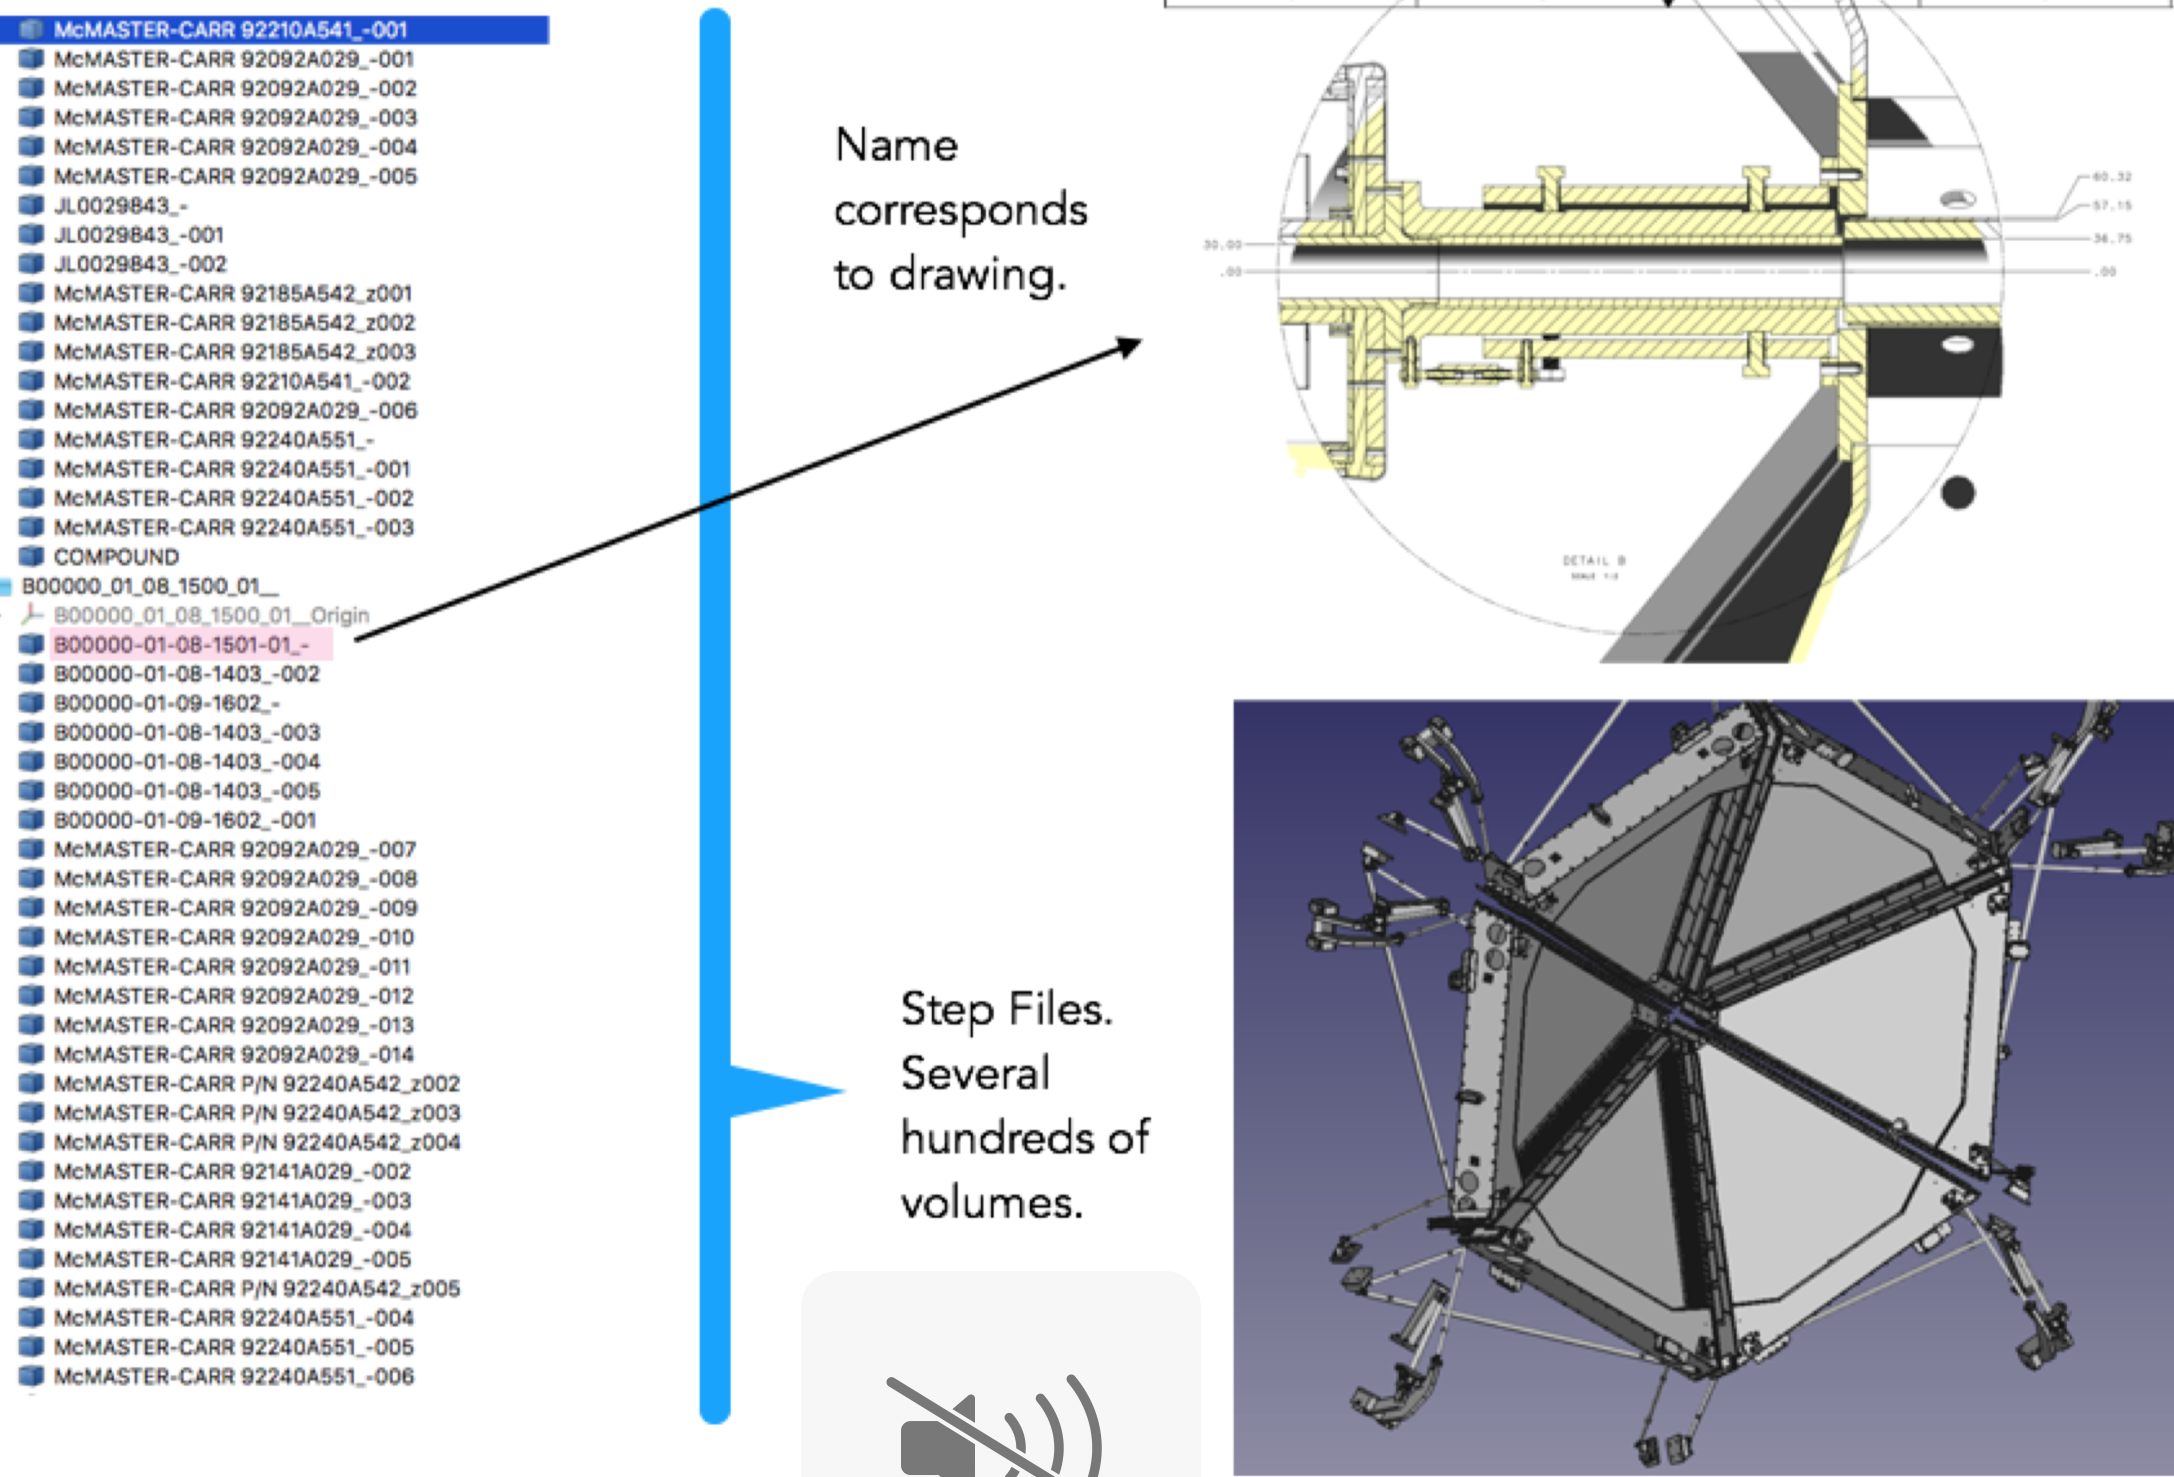
\includegraphics[width=0.98\columnwidth,keepaspectratio]{img/cadSelection.png}
	\caption{The selection of the volumes that will be used in the GEMC geant4 simulation.
             This typically involves filtering out unnecessary volumes that are not in the active region.}
	\label{fig:cadSelection}
\end{figure}

The elements in the STP file are then ``tessellated'': several polygon shapes are created to define a geant4 volume.
The software used to do this is FreeCad \cite{freeCad}. An example of tessellation showing the polygon shapes
is shown in \F{targetScatteringChamber}.

The simulated CAD import is as close to reality as the engineering model is close to reality.
We did encounter differences between the STP files, the drawings and reality in a few occasions and worked
out a workflow to eliminate any discrepancy, see \F{cadValidation}.


\begin{figure}
	\centering
	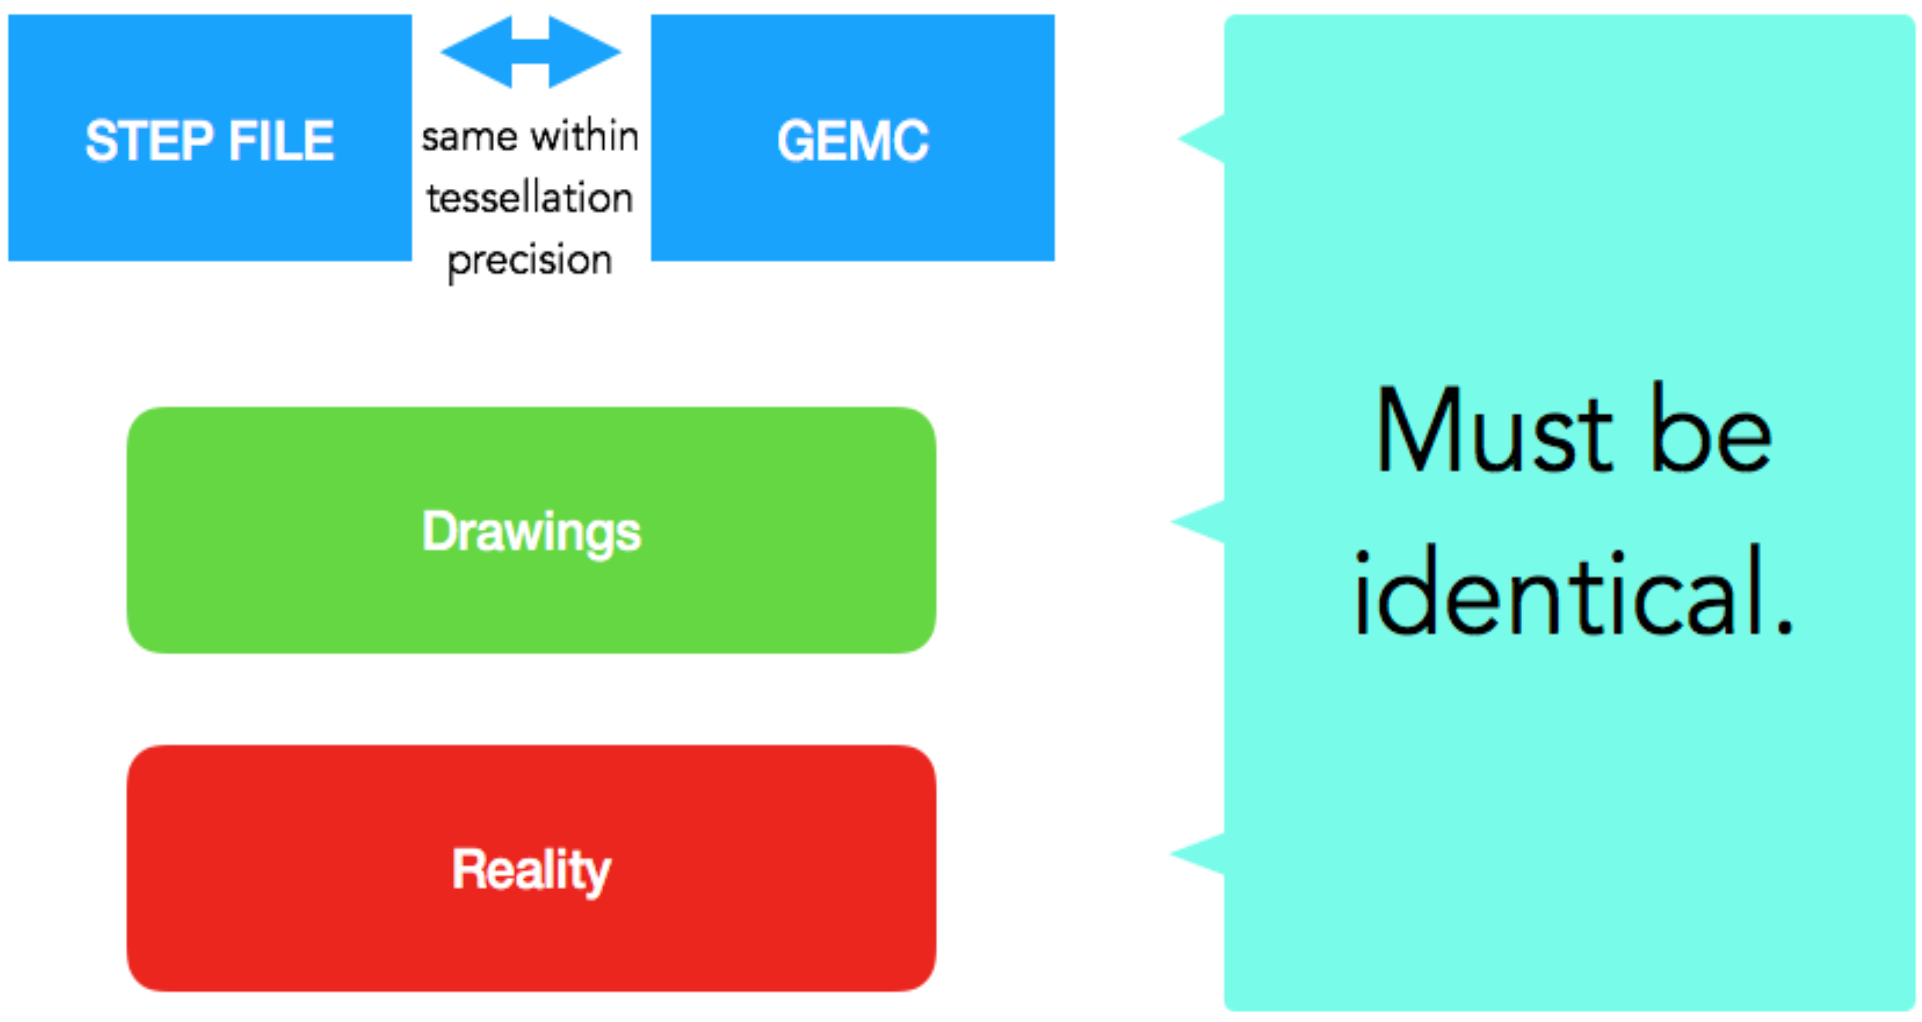
\includegraphics[width=0.95\columnwidth,keepaspectratio]{img/cadValidation.png}
	\caption{There are four possible representation of a volume: the one coming from the STP file
             and the tessellated one are exactly the same object (within the tessellation precision).
             In some cases, certain elements and their sizes and positions did not match the drawings.
             In other cases, they did not match what was built and measured, or their position did not
             match the survey. To eliminate these occurrences physicists and engineers worked until
             the final iteration of a volume was the same in all 4 models: STP/GEMC, Drawings and Reality}
	\label{fig:cadValidation}
\end{figure}

An example of the cad validation is shown in \F{cadValidationExample}.

\begin{figure}
	\centering
	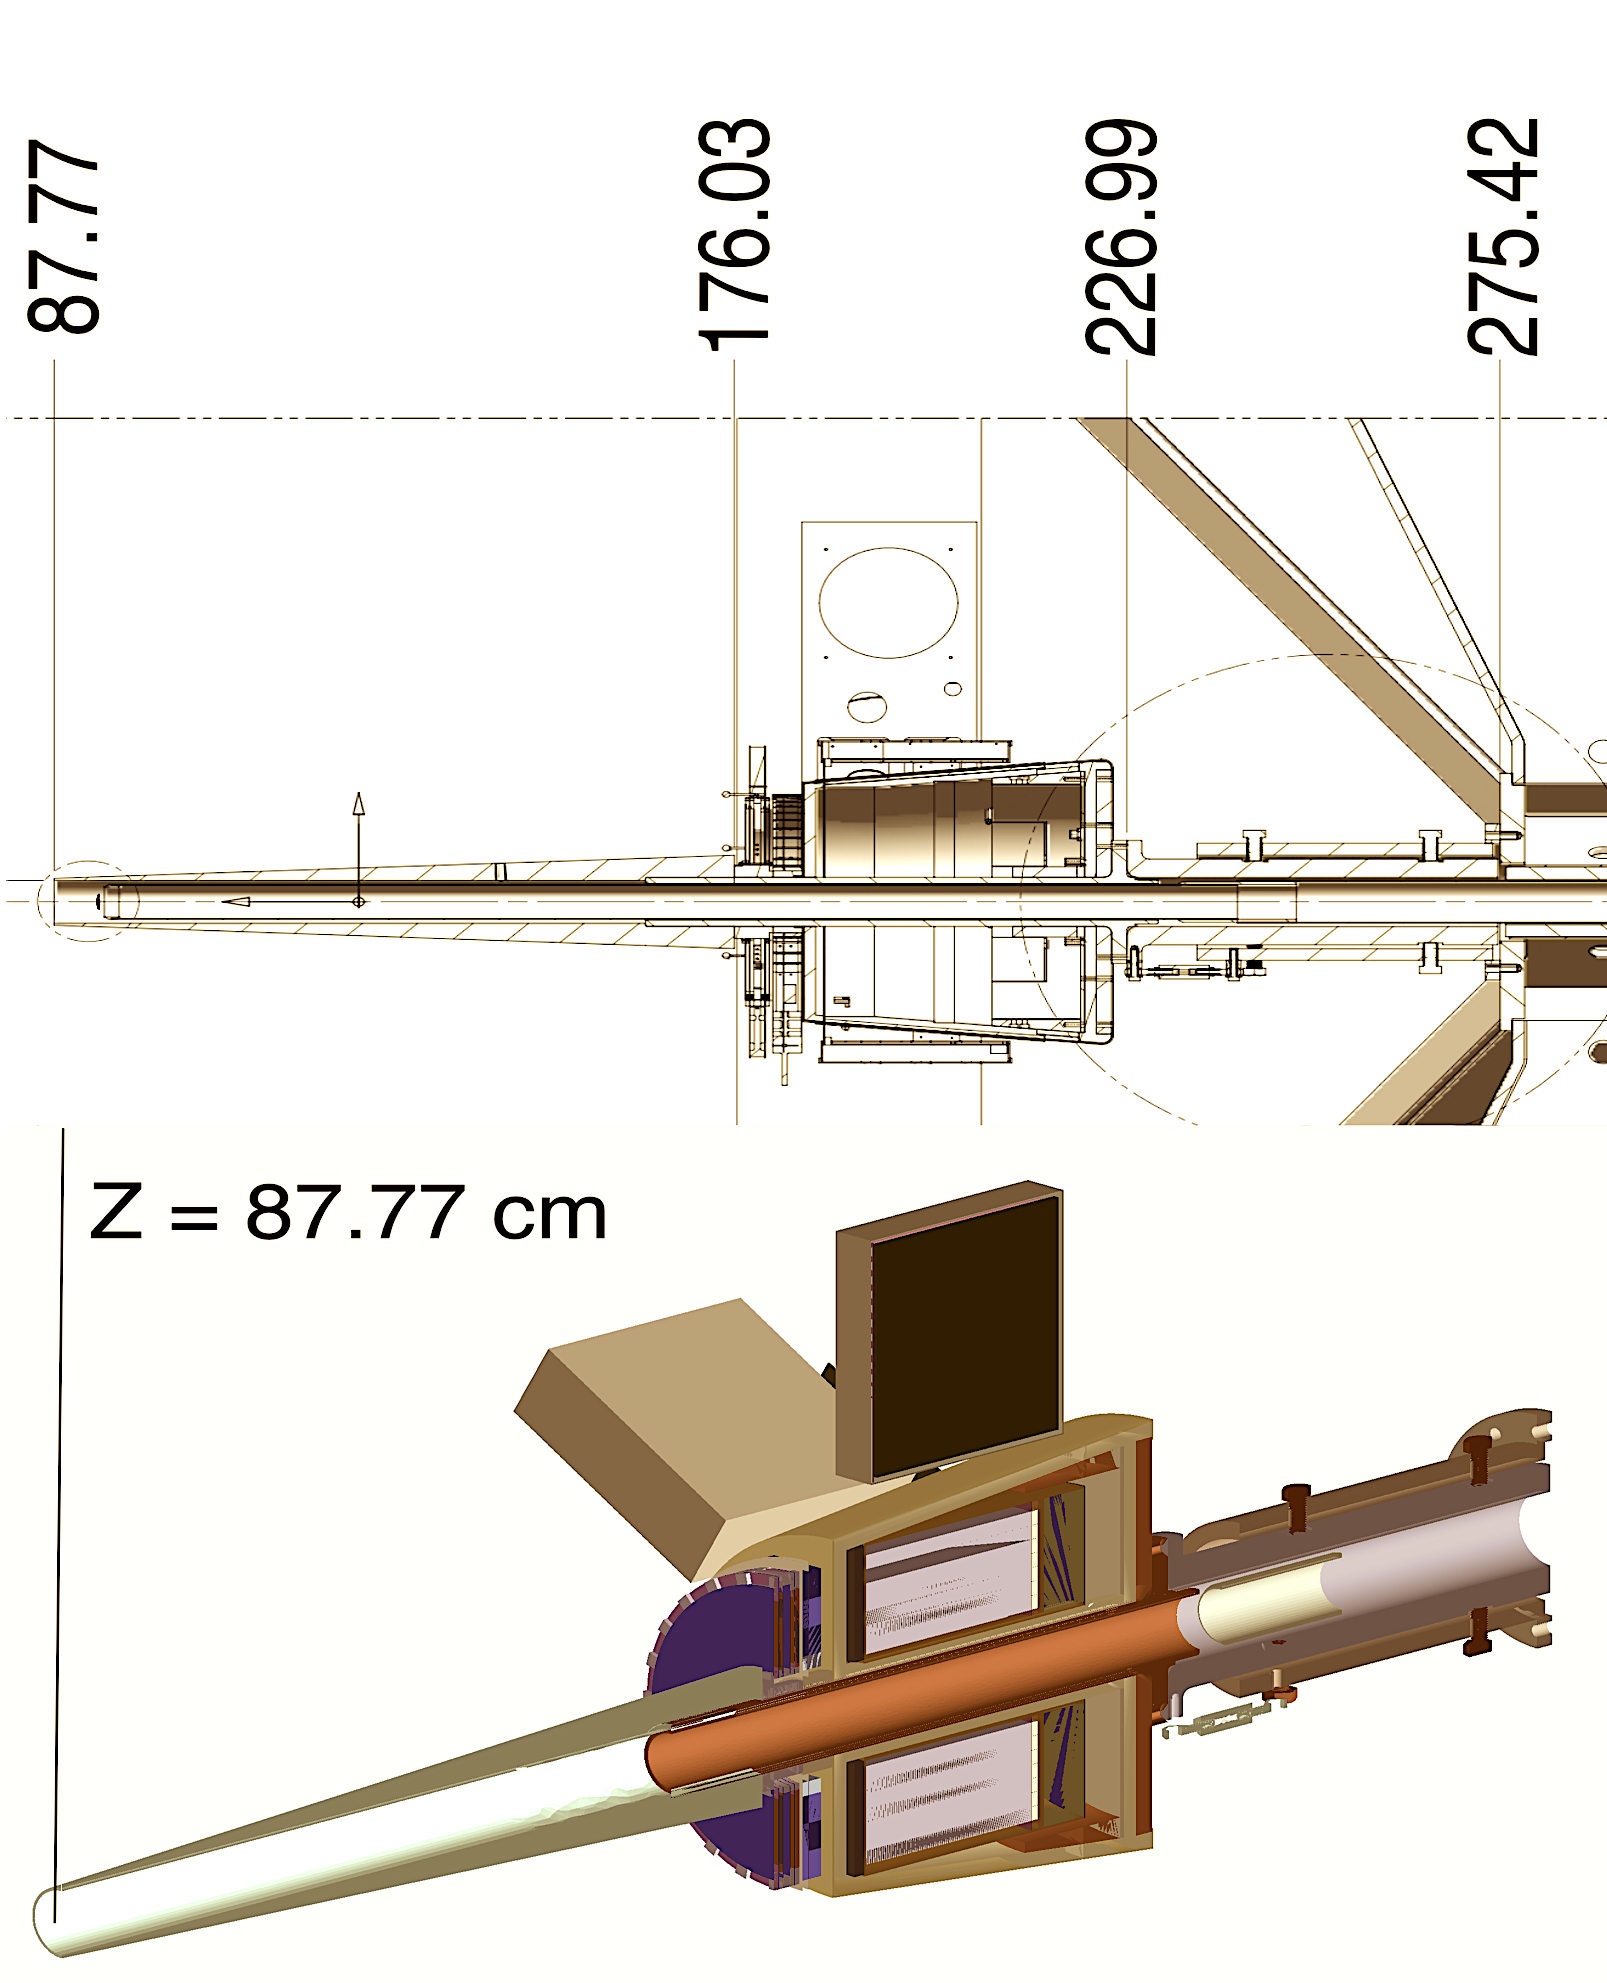
\includegraphics[width=0.95\columnwidth,keepaspectratio]{img/cadValidationExample.png}
	\caption{An example of comparing the gemc simulation to the drawings. Top: engineering drawings of
             the CLAS12 beamline and shielding. The start of the Moeller shielding is 87.77 cm downstream
             of the target center. Bottom: a geantino is shot vertically at z=87.77 cm, showing that the
             geant4 cone position agrees with the drawings.}
	\label{fig:cadValidationExample}
\end{figure}



\subsection{Magnetic Fields}
The magnetic fields are loaded from ascii files. The following geant4 parameters are loaded from
command line options or configuration files at run time:

\begin{itemize}
	\item minStep: minimum step in the magnetic field
	\item integralAlgorithm: compute the field value from the closest cell or using a linear interpolation
	\item interpolationMethod: interpolation algorithm, such as G4ClassicalRK4, G4SimpleRunge, etc
\end{itemize}

The implementation of the CLAS12 magnetic fields is described in \ref{clas12FieldMaps}.

\subsection{Detectors and Hit Process Plugins}
The detector are associated with c++ digitization routines at run time. This allows the routines to
be developed independently from the core code, and have 

\subsection{Event Time Window}

\subsection{Hit Definition}

\subsection{True Information}

\subsection{Database Constants}

\subsection{Process ID}

\subsection{Digitization}

\subsection{Output}

